\chapter{项目背景}
  LED产业发展迅速,在时装、新媒体艺术、纺织等领域,LED因其体积小、可靠性高、能耗低的特点,收到青睐,特别是柔性LED相关技术,更是亟待发展。
  
\chapter{研究计划}
目前将进行柔性电路的研究和测试,之后将分为以下几个应用场景进行开发:(不限于以下提出的应用场景)

{\heiti 应用场景1:脑电控制的交互式RGB-LED点阵穿戴式设备 }

通过检测脑电信号,将使用者的心情以Emoji等形式在休闲帽等穿戴式设备上用柔性LED阵列显示,从而达到交互的目的。

同时,穿戴式设备上的图案可以自定义,作为一种现代化的自我表达形式。还可以借助其他模块实现类似的附加功能,如:心率+呼吸+体温检测等。

由于柔性电路耐水洗且可靠,可以直接使用洗衣机清洗,做到了无负担的使用体验。相对于其他嵌入式的穿戴设备优势明显,消费者认同感较高。

相关技术:

TGAM脑电模块模块可以处理并输出脑波频率谱,脑电信号质量,原始脑电波和三个Neurosky的eSense参数:专注度,放松度和眨眼侦测。由于能耗小且和人体的界面只需一个简单的干接触点,所以可以适合运用于柔性穿戴式设备中。

{\heiti 应用场景2:用于摄影行业的柔性LED平板 }

目前,摄影界普遍应用的摄影垫,制作工艺往往是LED灯带平铺在柔性材料上面,可靠性和成本低廉不可兼得,且色调单一。若应用柔性LED制作照明平板,不仅可靠性大大提升,而且柔性LED良好的性能可以实现更多的应用,如制作高尼特的球形光源等。

另外,对于个人用户的diy摄影创作,单一色源以及照射方式的摄影补光难以满足需求。柔性led照明设施能够很好地达到一种补光光源个性化定制的的效果

\chapter{类似产品分析}  
\section{The Embroidered Computer——刺绣计算机}
刺绣计算机是Irene Posch探索使用历史金刺绣材料和知识来制作可编程8位计算机。

http://www.ireneposch.net/

该产品仅由各种金属线,磁性,玻璃和金属珠子构成,并受到传统制作程序和图案的启发,对我们周围的当前数字和电子技术的外观以及我们与它们的互动提出质疑。

从技术上讲,该产品由(纺织)继电器组成,类似于半导体发明之前的早期计算机。在视觉上,金材料,这里用于它们的导电性能,排列成特定的图案以实现电子功能,主导着工作。传统上纯粹是装饰性的,这里的图案定义了它们的功能。它们裸露的核心数字例程通常隐藏在黑盒子里。邀请用户与编织纺织品的部分进行交互以为其计算。

%\begin{figure}
%\begin{minipage}{0.48\textwidth}
%  \centering
%  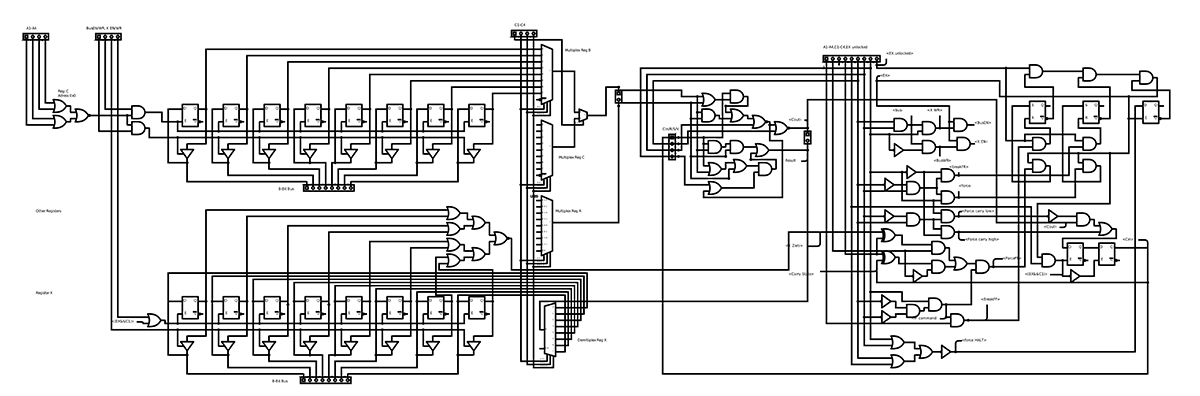
\includegraphics[height=4cm]{logic-diagram-controll-unit-1_small.jpg}
%  \caption{逻辑电路图}
%  \label{cube}
%\end{minipage}\hfill
%\begin{minipage}{0.48\textwidth}
%  \centering
%  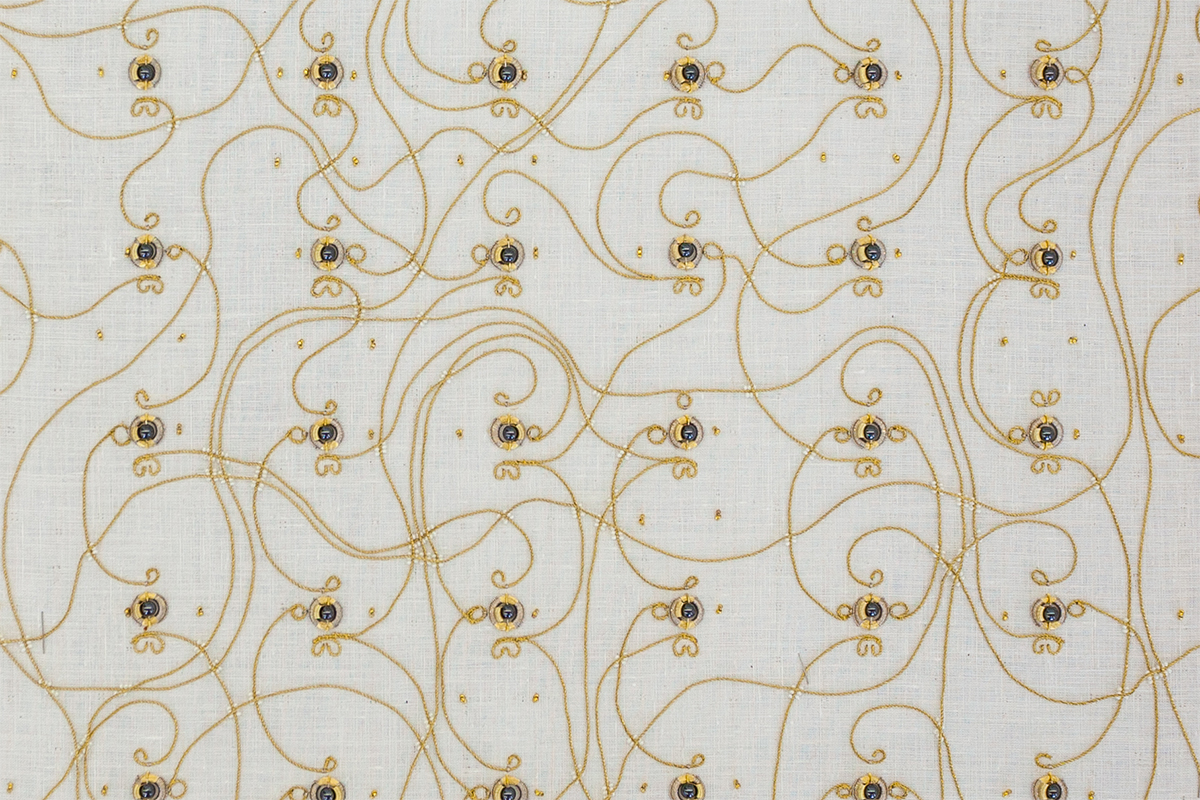
\includegraphics[height=4cm]{MG_0411_size_detail_web.jpg}
%  \caption{刺绣计算机}
%  \label{tri}
%\end{minipage}
%\end{figure}

\begin{figure}[htbp]
\centering
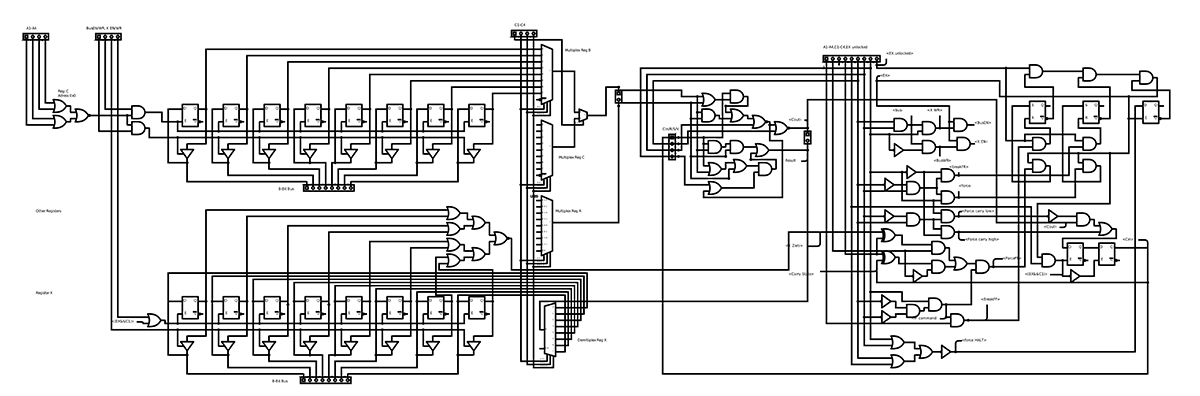
\includegraphics[width=10cm]{logic-diagram-controll-unit-1_small.jpg}
\caption{逻辑电路图} 
\label{1}
\end{figure}

\begin{figure}[htbp]
\centering
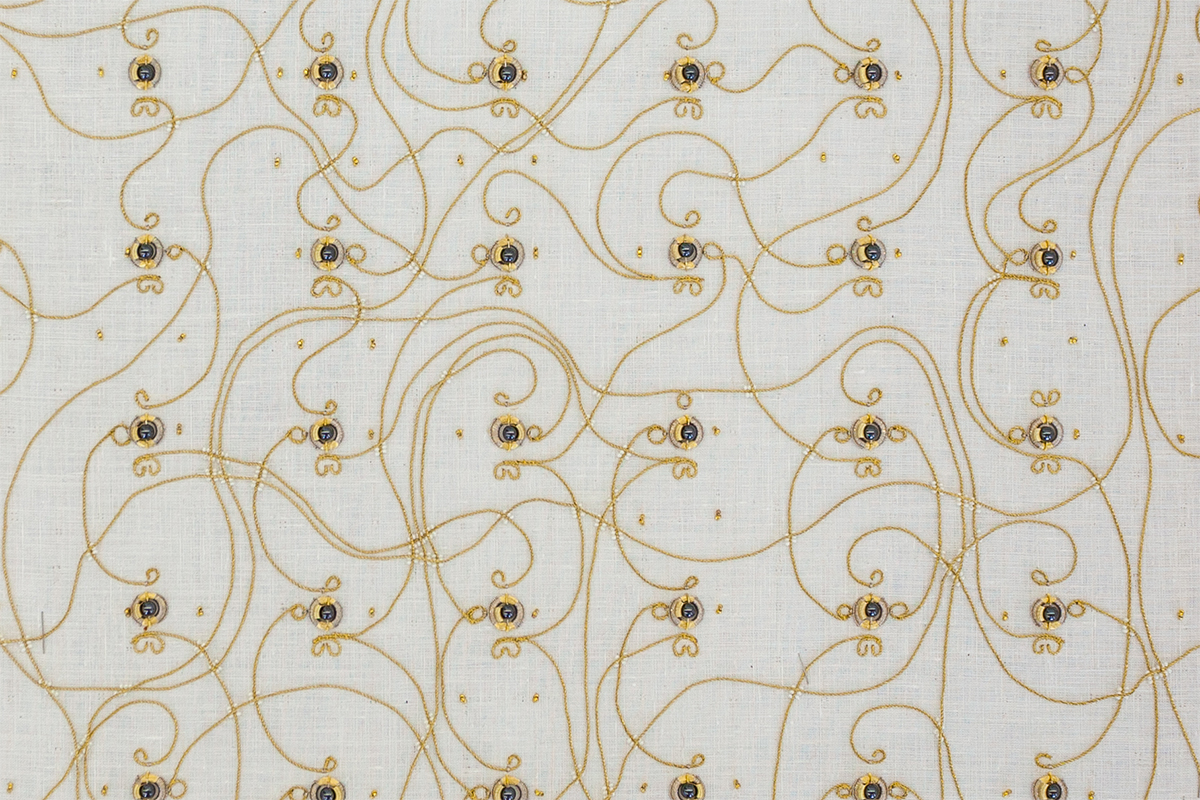
\includegraphics[width=10cm]{MG_0411_size_detail_web.jpg}
\caption{刺绣计算机} 
\label{2}
\end{figure}


由于其基本元件(门)均为继电器形式,固只能作为展品展示,无法抗冲击,但其电气链接可以供我们参考。

\newpage

\section{PIX}
PIX是一款嵌入半柔性LED面板的背包。

Pix Backpack的设计旨在让日常生活更加美好。 它结合了方便的都市背包和灵活的可编程屏幕。通过免费的IOS / Android应用程序控制Pix。 你可以在app里找到各种各样的图片/动画/小工具和游戏。只需选择你喜欢的内容,一键上传到Pix背包。

作为一款个性化背包,其设计非常个性化。但是PIX采用的不是真正柔性的LED,而是在栅格状的泡沫中嵌入LED灯,他的发光平面不能折叠且较为厚重,但在书包这一应用场景中不是一个很大的问题。

https://www.pix.style/

\begin{figure}[htbp]
\centering
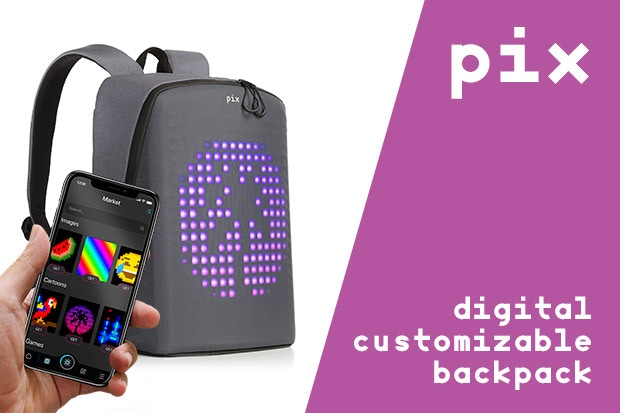
\includegraphics[width=10cm]{pix.jpg}
\caption{PIX} 
\label{p1}
\end{figure}

\section{e-broidery}

e-broidery照明纺织品保证了日夜的迷人印象。集成电子设备可实现暗淡功能和动画。 LED纺织品可以洗涤和悬垂。此外,还保留了基础面料的悬挂特性和质地 - 无论是薄纱还是厚重的织物。

除了标准产品之外,照明纺织品可以由预定的织物和刺绣选择构成。还提供基于个人客户请求的定制。包括:预选面料、刺绣、设计和灯光图案以及亮度水平等。

可以说e-broidery很好的实现了单色LED灯在织物上的嵌入,但是e-broidery并没有加入较复杂的控制(比如只有灯的闪烁控制而没有RGB控制),而且织物中只有单一型号的LED。另外e-broidery的价格十分昂贵,大约2000欧元/平方米,所以目前只有高端时装界和摄影界在使用。


\begin{figure}[htbp]
\centering
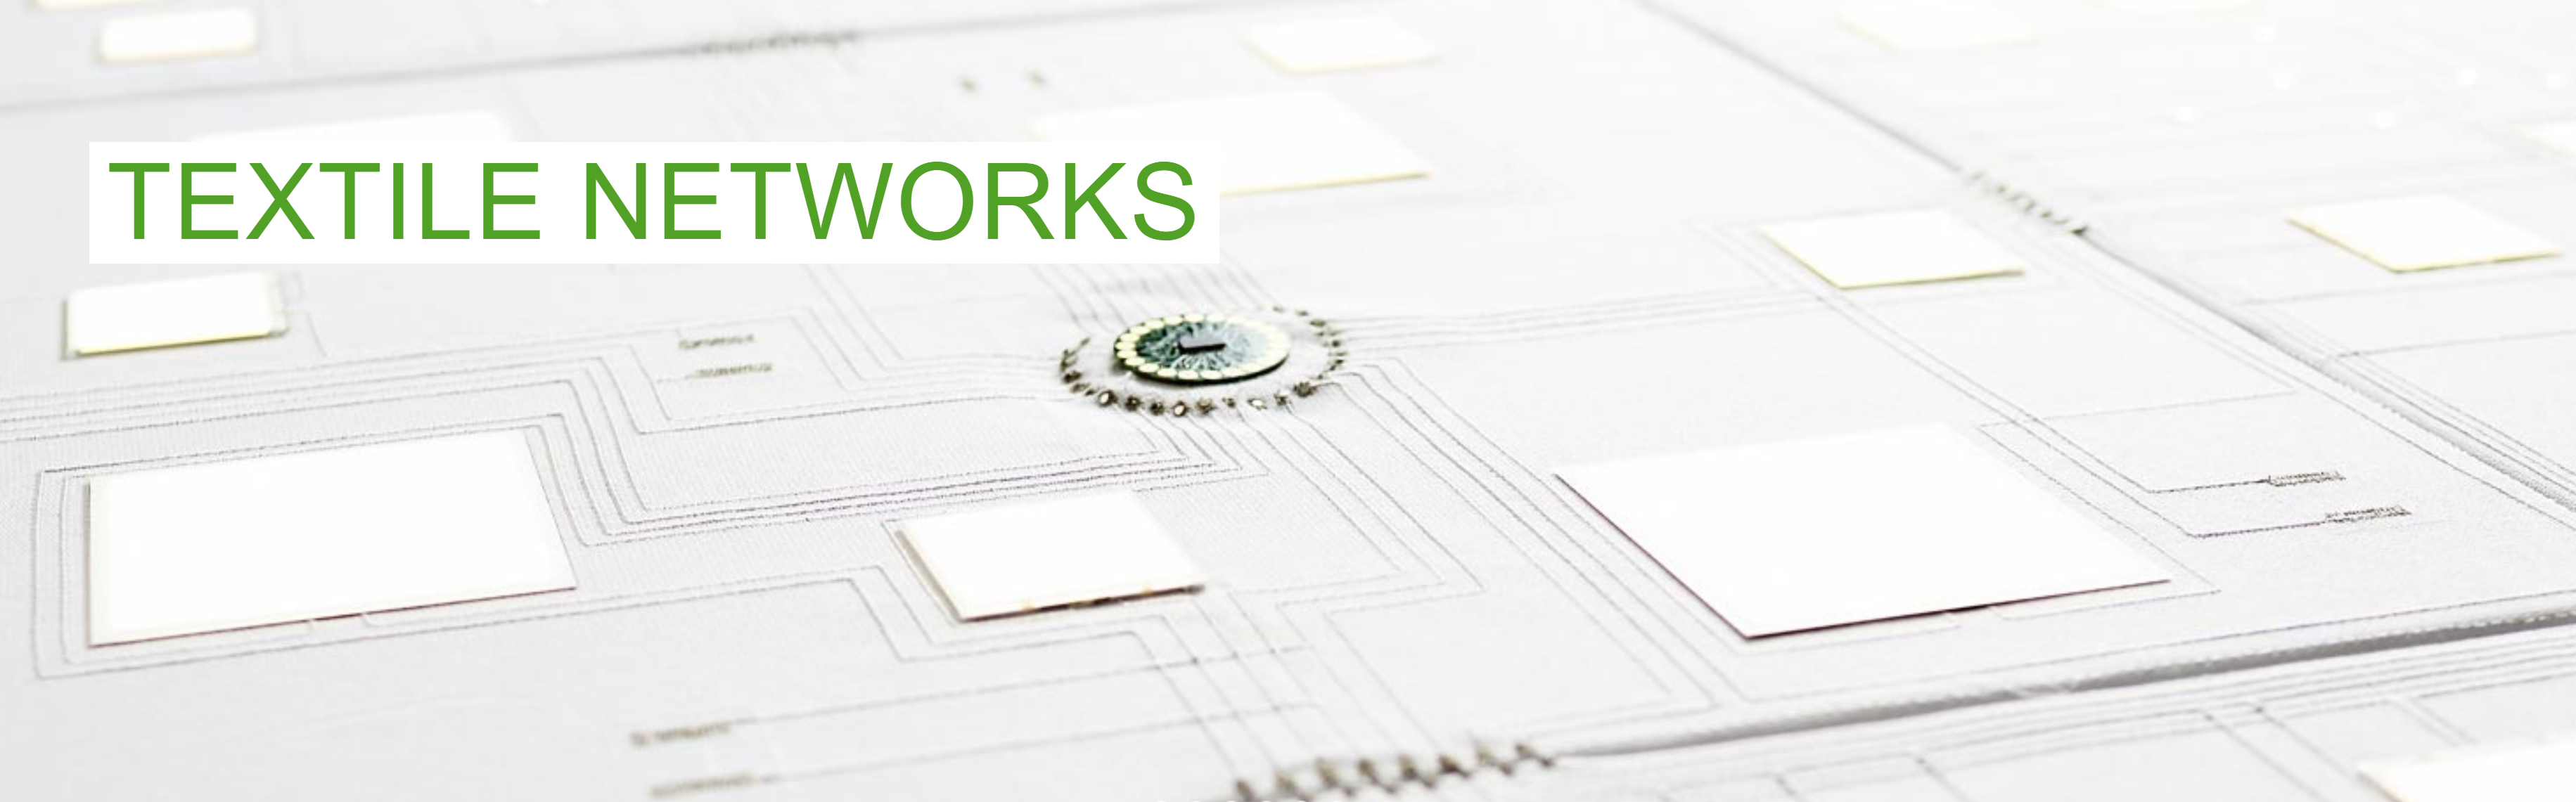
\includegraphics[width=10cm]{textile.png}
\caption{e-broidery效果图} 
\label{e1}
\end{figure}

\begin{figure}[htbp]
\centering
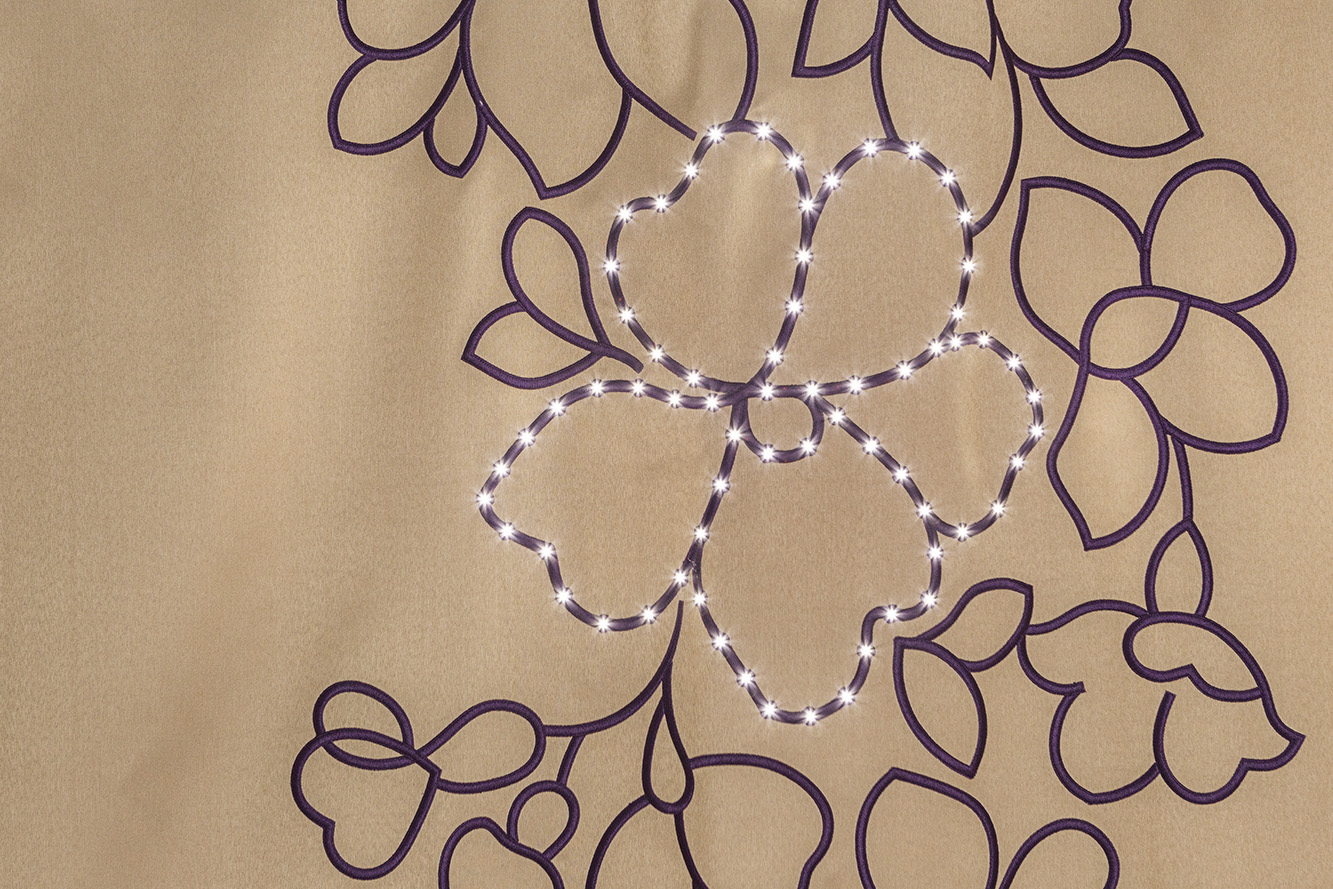
\includegraphics[width=10cm]{DIMOUT-MATT-BOUQUET_camel_WEB.jpg}
\caption{e-broidery制成的时装布料} 
\label{e2}
\end{figure}

http://www.frti.ch/en/

http://www.e-broidery.ch/en/


\chapter{技术方案}

\chapter{实现}
\chapter{展望}


%\subsection{}